\begin{figure}[tb]
\begin{center}
\setlength{\tabcolsep}{0pt}
\newcommand\figwidth{.22}
%
\begin{tabular*}{0.92\textwidth}{c @{\extracolsep{\fill}} cccc}
    \rotatebox[origin=c]{90}{Train}
    &
    \raisebox{-0.45\height}{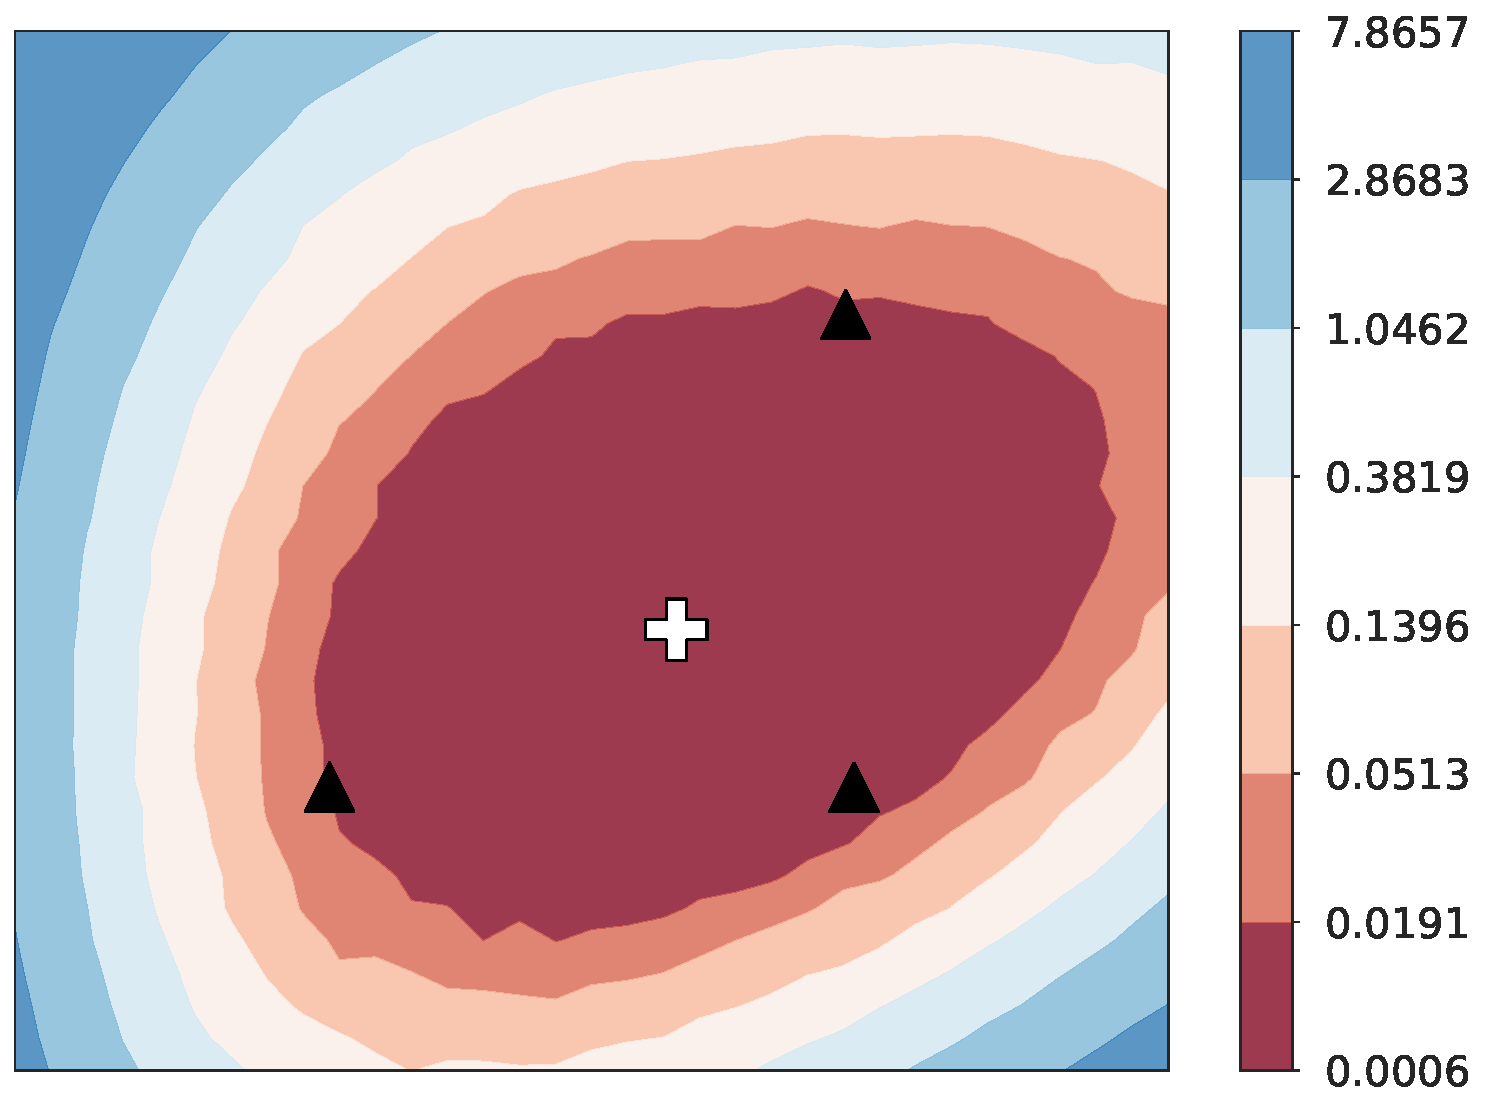
\includegraphics[width=\figwidth\textwidth]{figures/loss_surfaces/TE0_in_loss_plane.pdf}}
    &
    \raisebox{-0.45\height}{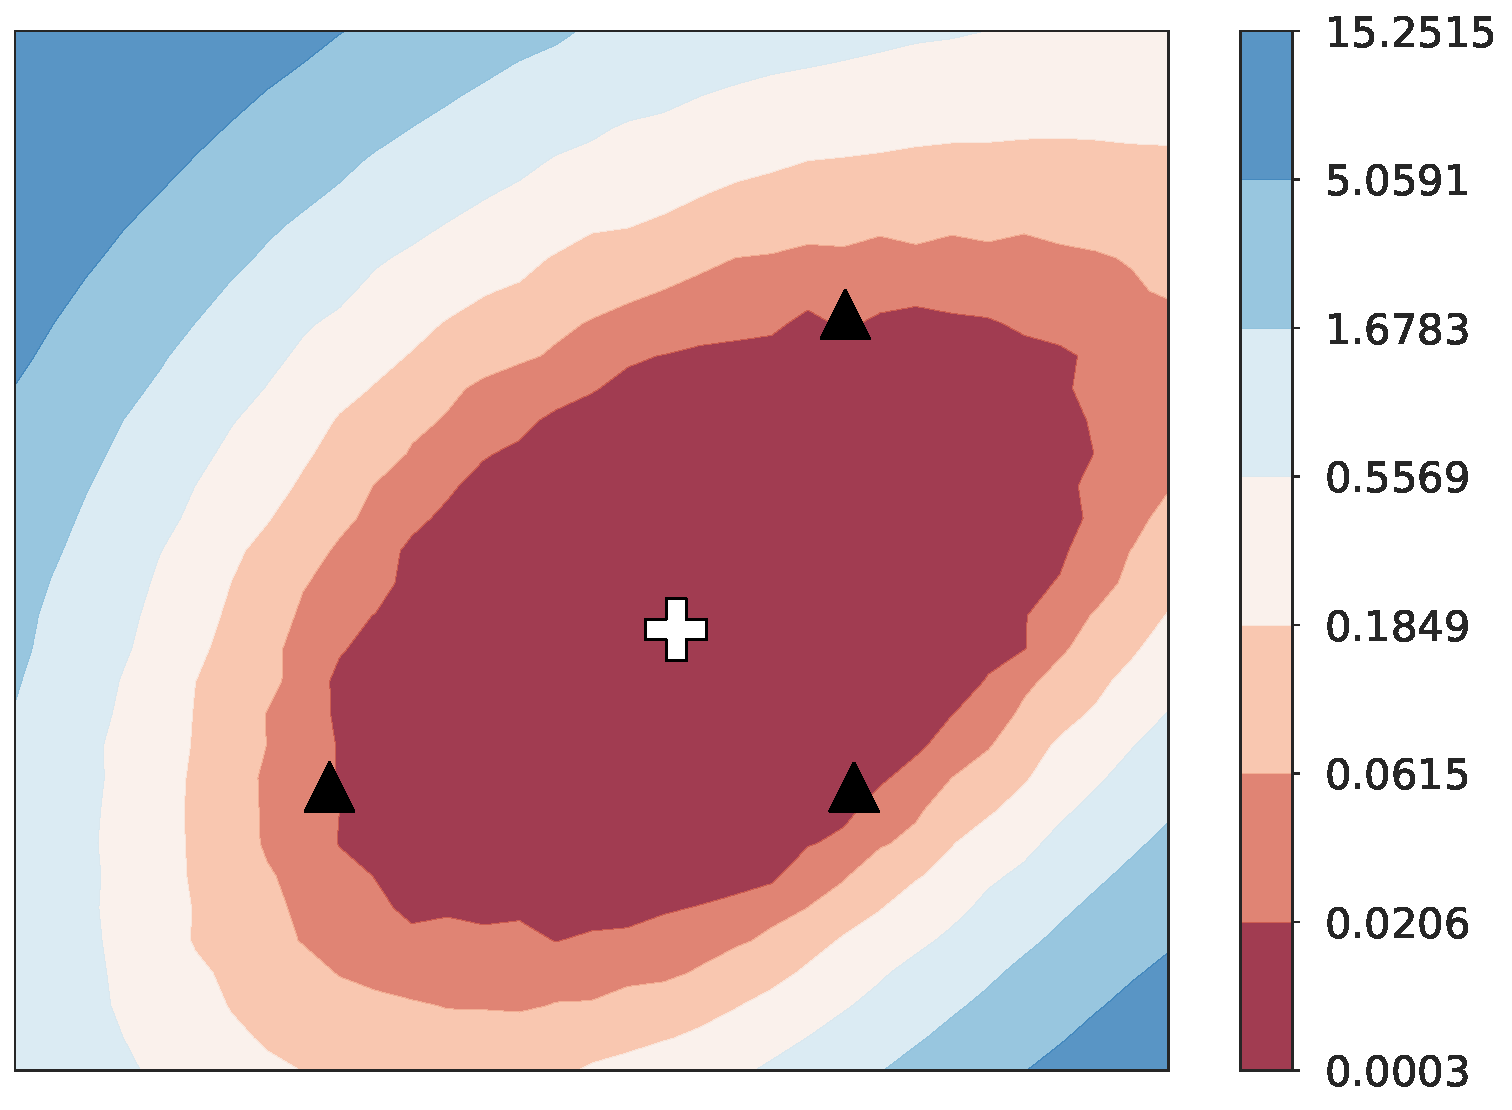
\includegraphics[width=\figwidth\textwidth]{figures/loss_surfaces/TE1_in_loss_plane.pdf}}
    &
    \raisebox{-0.45\height}{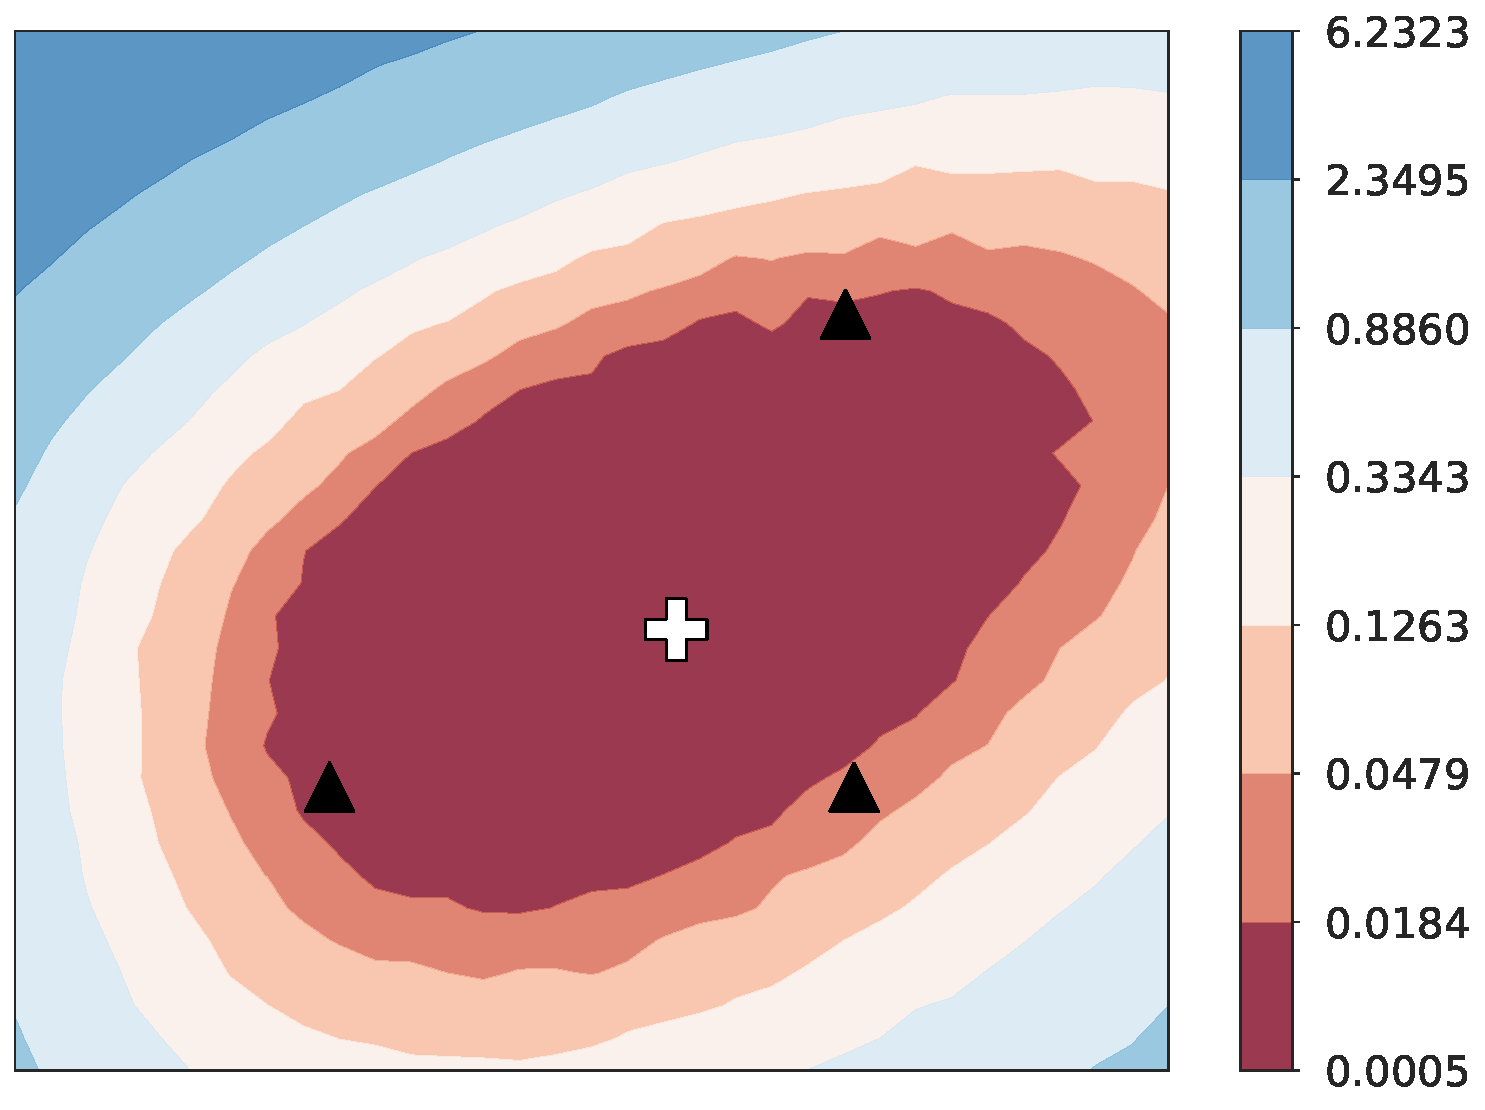
\includegraphics[width=\figwidth\textwidth]{figures/loss_surfaces/TE2_in_loss_plane.pdf}}
    &
    \raisebox{-0.45\height}{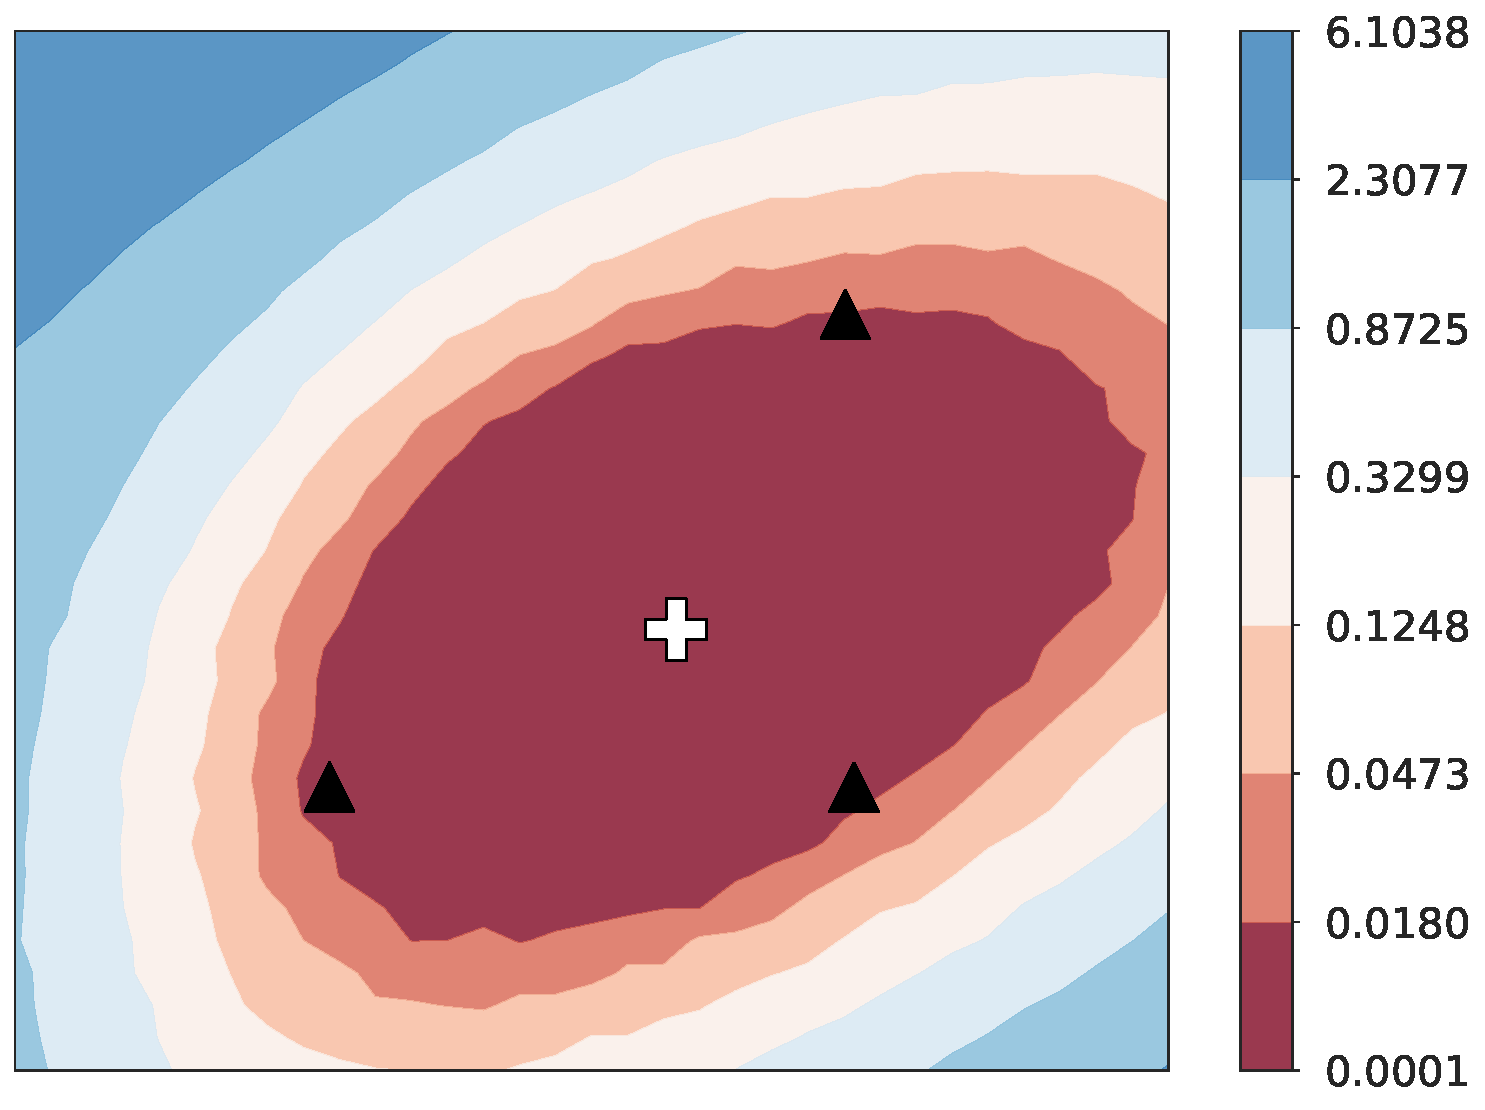
\includegraphics[width=\figwidth\textwidth]{figures/loss_surfaces/TE3_in_loss_plane.pdf}}
\\
    \rotatebox[origin=c]{90}{Test}
    &
    \raisebox{-0.5\height}{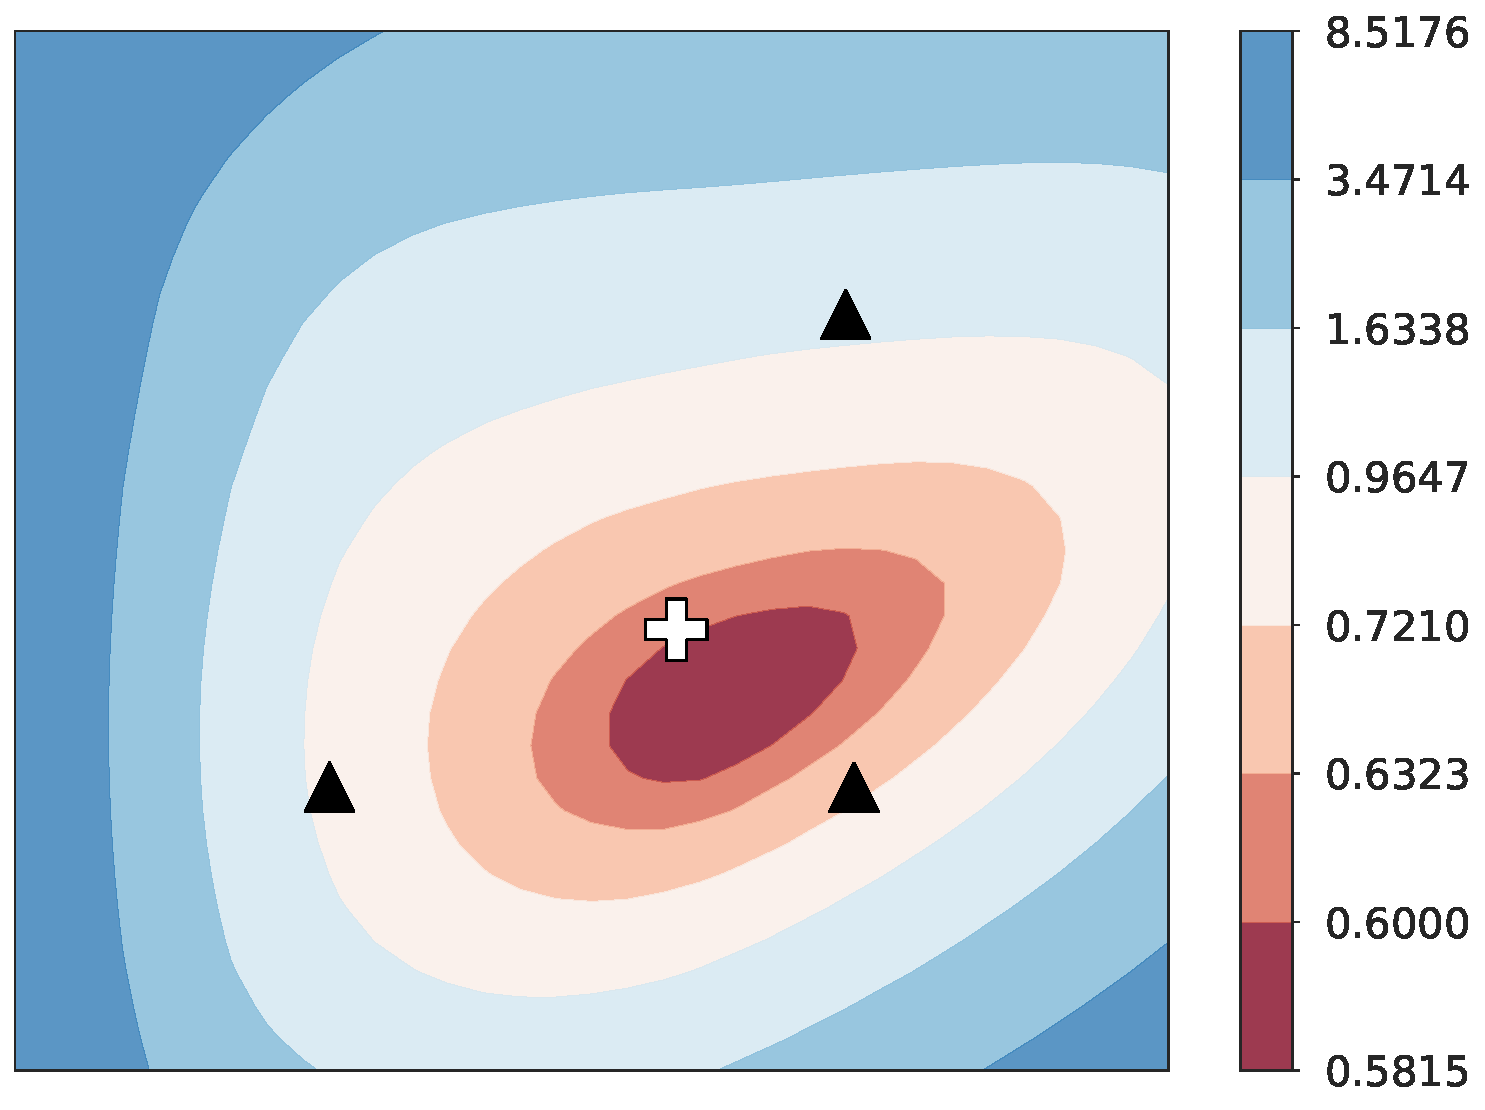
\includegraphics[width=\figwidth\textwidth]{figures/loss_surfaces/TE0_env0_in_loss_plane.pdf}}
    &
    \raisebox{-0.5\height}{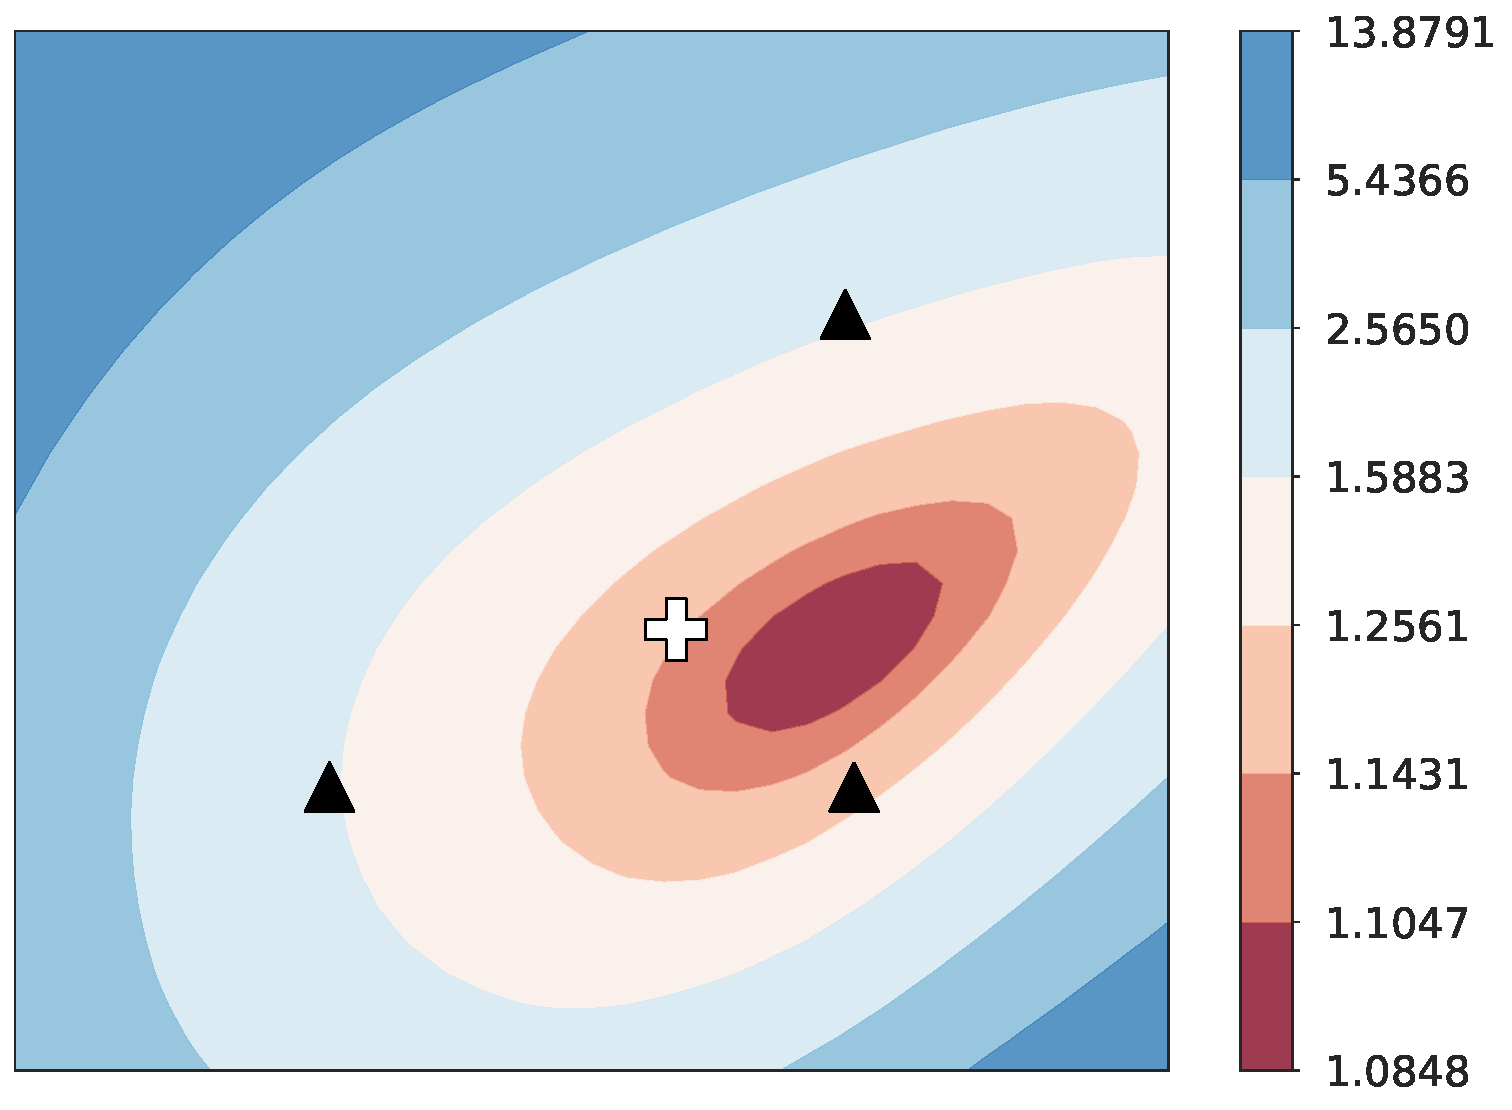
\includegraphics[width=\figwidth\textwidth]{figures/loss_surfaces/TE1_env1_in_loss_plane.pdf}}
    &
    \raisebox{-0.5\height}{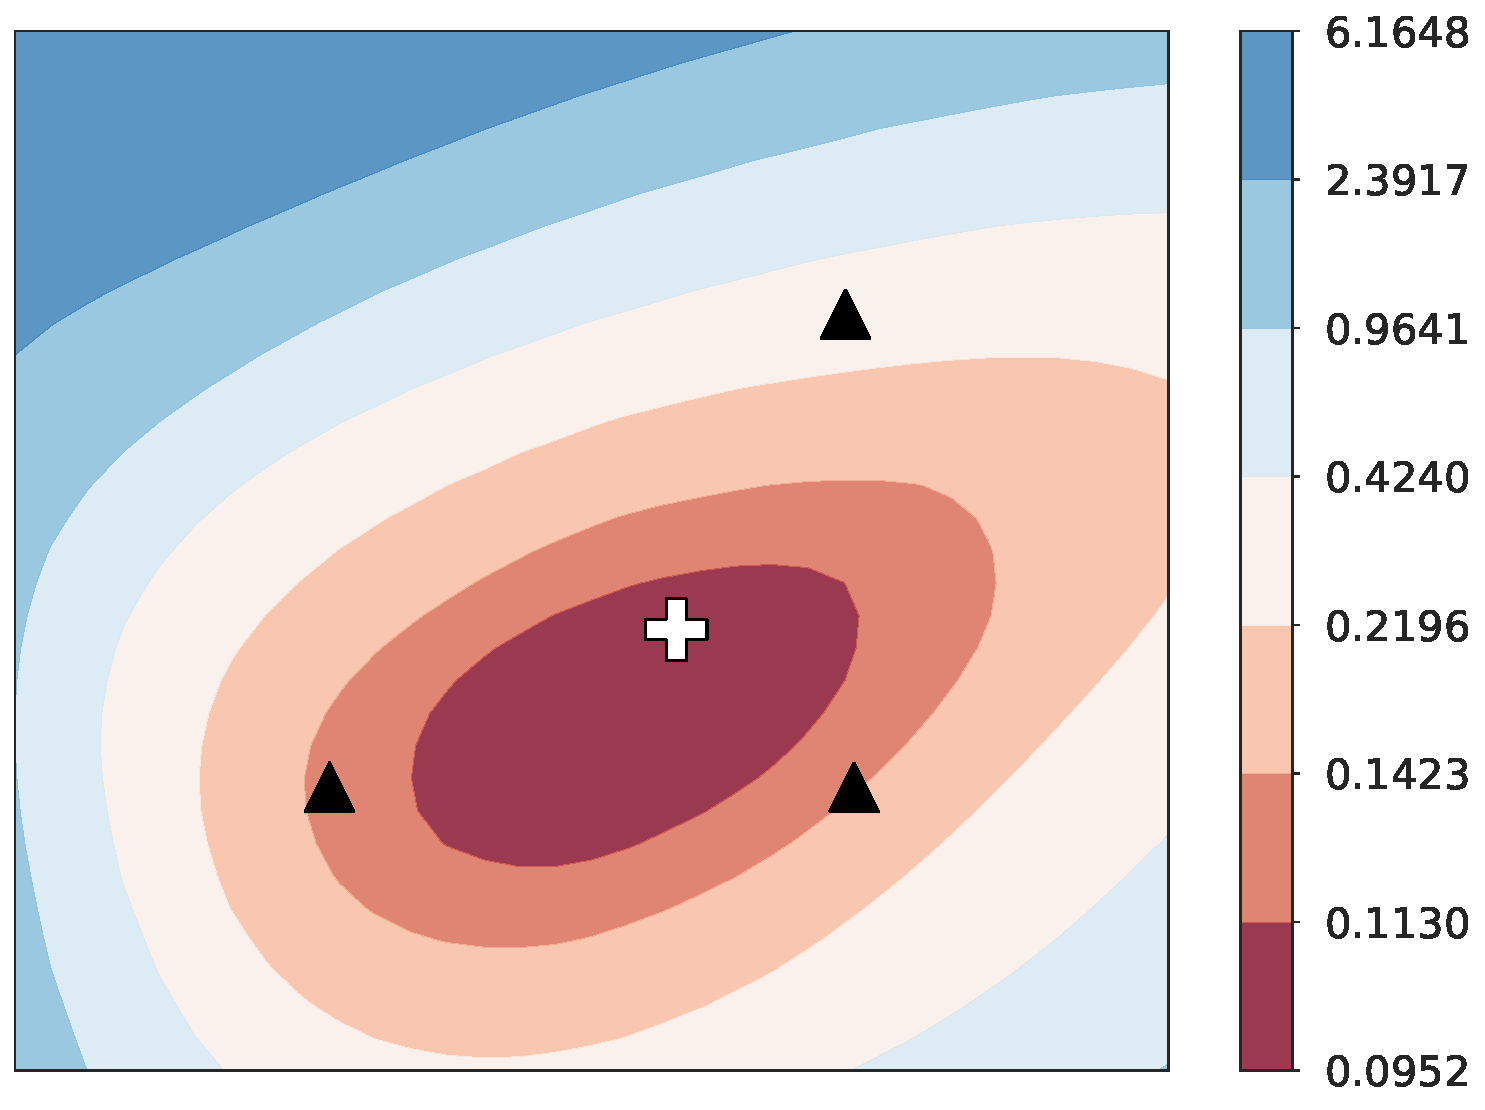
\includegraphics[width=\figwidth\textwidth]{figures/loss_surfaces/TE2_env2_in_loss_plane.pdf}}
    &
    \raisebox{-0.5\height}{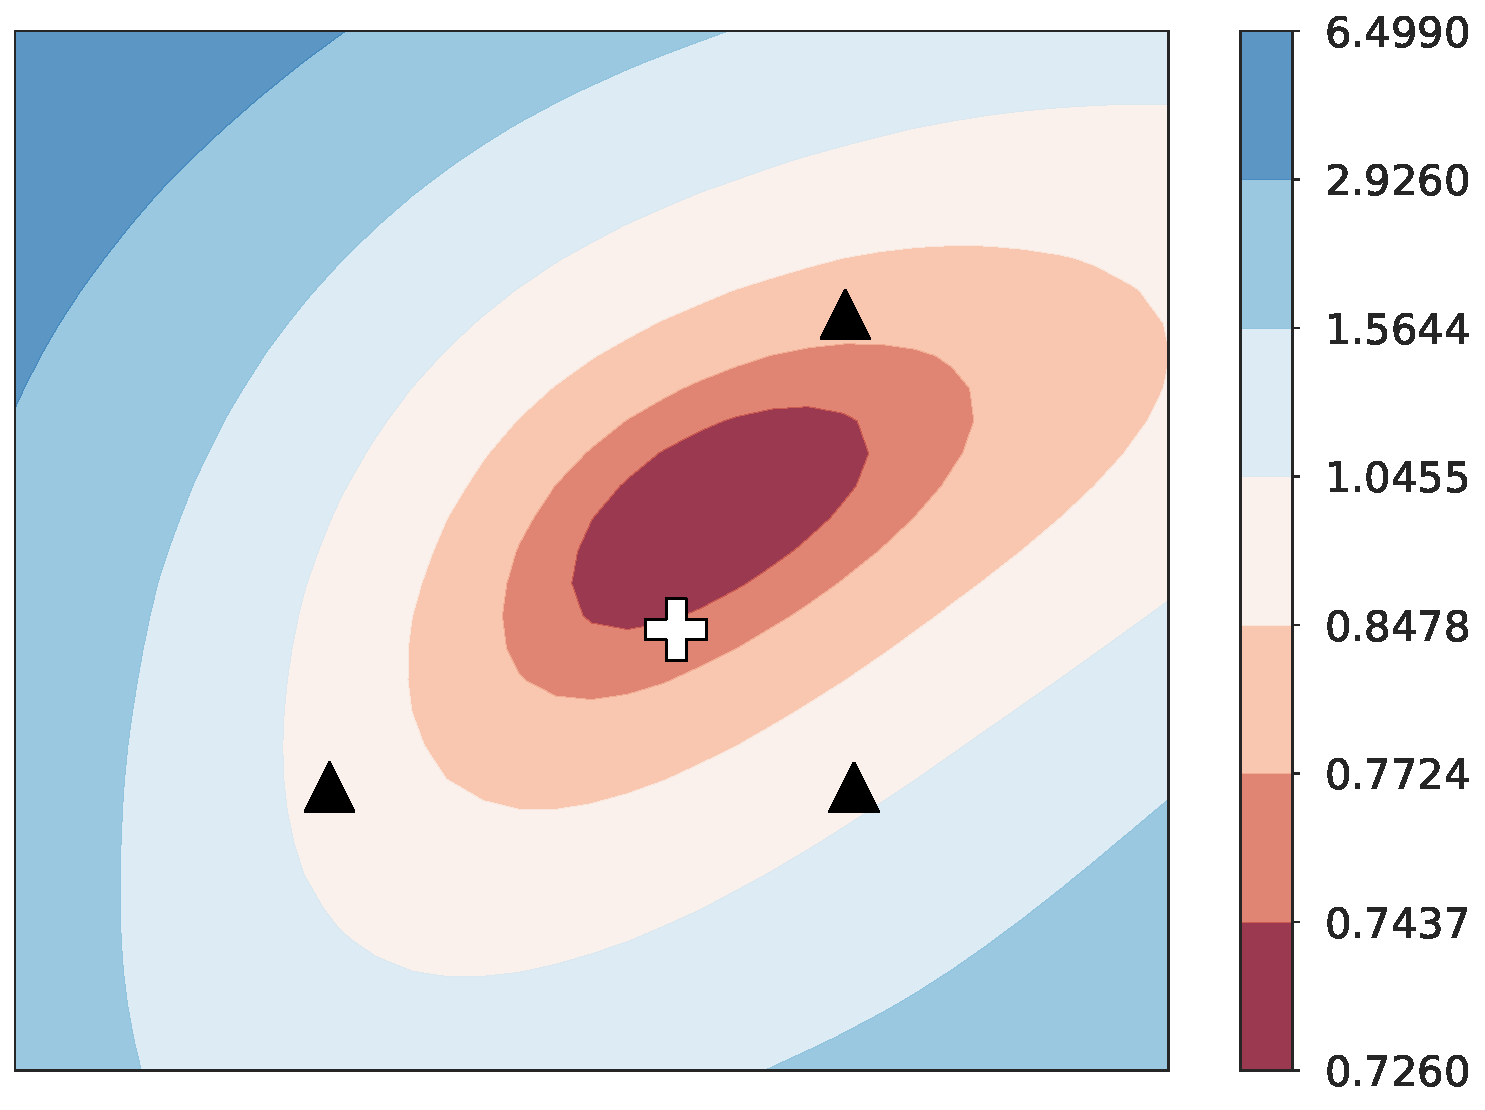
\includegraphics[width=\figwidth\textwidth]{figures/loss_surfaces/TE3_env3_in_loss_plane.pdf}}
\\
    &
    {\small \textit{Art painting} (test)}
    &
    {\small \textit{Cartoon} (test)}
    &
    {\small \textit{Photo} (test)}
    &
    {\small \textit{Sketch} (test)}
\end{tabular*}
%
\end{center}
\vspace{-0.5em}
\caption{\small \textbf{Loss surfaces on model parameters in \data{PACS} dataset for each target domain.} 
The three triangles indicate model weights chosen at the end of training phase with equal intervals. Each plane is defined by the three weights and losses upon the plane are visualized with contours. The center cross mark is averaged point of the three weights. The first and second rows show the averaged training loss and the test loss surfaces, respectively.
% \sr{coloring the center yellow?}
}
\vspace{-0.5em}
\label{fig:loss_space}
\end{figure}




% \iffalse

% % vertically centering
% \begin{figure*}[t]
% \centering
% %\raggedright
% \captionsetup[subfigure]{aboveskip=0pt,belowskip=0pt}
% \begin{subfigure}[b]{0.24\textwidth}
%     
\includegraphics[width=\textwidth]{figures/all_loss_surfaces/PACS/TE0_in_loss_plane.pdf}
%     % \caption{\textit{Art painting} (valid)}
% \end{subfigure}
% \begin{subfigure}[b]{0.24\textwidth}
%     
\includegraphics[width=\textwidth]{figures/all_loss_surfaces/PACS/TE1_in_loss_plane.pdf}
%     % \caption{\textit{Cartoon} (valid)}
% \end{subfigure}
% \begin{subfigure}[b]{0.24\textwidth}
%     
\includegraphics[width=\textwidth]{figures/all_loss_surfaces/PACS/TE2_in_loss_plane.pdf}
%     % \caption{\textit{Sketch} (valid)}
% \end{subfigure}
% \begin{subfigure}[b]{0.24\textwidth}
%     
\includegraphics[width=\textwidth]{figures/all_loss_surfaces/PACS/TE3_in_loss_plane.pdf}
%     % \caption{\textit{Photo} (test)}
% \end{subfigure}
% \\
% % \raggedright
% \begin{subfigure}[b]{0.24\textwidth}
%     
\includegraphics[width=\textwidth]{figures/all_loss_surfaces/PACS/TE0_env0_in_loss_plane.pdf}
%     \caption{\textit{Art painting} (test)}
% \end{subfigure}
% \begin{subfigure}[b]{0.24\textwidth}
%     
\includegraphics[width=\textwidth]{figures/all_loss_surfaces/PACS/TE1_env1_in_loss_plane.pdf}
%     \caption{\textit{Cartoon} (test)}
% \end{subfigure}
% \begin{subfigure}[b]{0.24\textwidth}
%     
\includegraphics[width=\textwidth]{figures/all_loss_surfaces/PACS/TE2_env2_in_loss_plane.pdf}
%     \caption{\textit{Photo} (test)}
% \end{subfigure}
% \begin{subfigure}[b]{0.24\textwidth}
%     
\includegraphics[width=\textwidth]{figures/all_loss_surfaces/PACS/TE3_env3_in_loss_plane.pdf}
%     \caption{\textit{Sketch} (test)}
% \end{subfigure}

% \vspace{-0.5em}
% \caption{\textbf{Loss surfaces on model parameters in \data{PACS} dataset for each target domain. 
% %In-distribution loss surface when target domain is \textit{photo} in PACS dataset.
% } 
% The three points such as circle, rectangle, and triangle indicate model weights chosen at the end of training phase with equal intervals. Each plane is defined by the three weights and losses upon the plane are visualized with contours. First and second rows show the averaged training loss and the test loss surfaces, respectively.\sr{put ``in-domain loss'' and ``out-of-domain loss'' on the left}}
% \vspace{-1.0em}
% \label{fig:loss_space}
% \end{figure*}

% \fi
